\documentclass{article}
\author{Tyler Compton}
\title{Section 10.3 - Dot Product}

\usepackage{graphicx}
\usepackage{float}
\usepackage{amsfonts}
\usepackage{gensymb}
\usepackage{amsmath}
\usepackage{esvect}
\graphicspath{ {images/} }

\begin{document}

\maketitle
\tableofcontents

\section{Introduction}
In the last section, we discussed how one may add and subtract vectors, as well
as how to multiply a vector by a scalar. However, we never mentioned how two
vectors can be multiplied. In this section, we discuss one of the ways this can
be done.

The dot product is a mathematical operator that works on two vectors and
produces a scalar. It is represented by a dot, like so:

$$<1, 2, 3> \cdot <4, 5, 6>$$

The dot product is calculated by summing the products of each vector component.
For a $\mathbb{R}^3$ vector, the formula would look like this:

$$\vv{a} \cdot \vv{b} = a_1b_1 + a_2b_2 + a_3b_3$$

The subscripts represent a single component of the vector. For the vector
$a = <3, 4, 5>$, $a_2 = 4$.

\section{Dot Product Value}
The value of the dot product can give us insight about the relationship between
two vectors. The dot product can tell us the kind of angle the two vectors
create.

\begin{table}[H]
	\centering
	\begin{tabular} { l l }
		Dot Product & Angle Type
		$0<dot$ & Acute
		$0>dot$ & Obtuse
		$0=dot$ & Right
	\end{tabular}
\end{table}

This provides a way to test if two vectors are perpendicular, or orthagonal.

\section{Second Dot Product Form}
The sum-of-component-products dot product form can tell us some basic
information about the angle between two vectors, but it tells us very little
about the value of that angle if it isn't $90\degree$. To find the specific
angle value, we need to use another dot product relationship.

$$\vv{a} \cdot \vv{b} = \left|\vv{a}\right| \left|\vv{b}\right| cos(\theta)$$

One could technically solve for the dot product using this method if they
happened to know the magnitude of $\vv{a}$ and $\vv{b}$ and the angle they
make, but that is not a common scenario. The more useful application for this
relationship is to find the dot product using the original form and solve for
$\theta$.

\section{Projecting Vectors}
Imagine two vectors that have a non-zero angle value between them. Now imagine
shining a light over the top of the upper vector. The upper vector would cast a
shadow straight down onto a piece of the lower vector. What if we wanted to
find the vector value of that piece?

\begin{figure}[H]
	\centering
	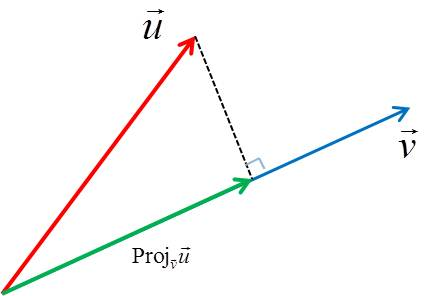
\includegraphics[width=6cm]{projection}
	\caption{A graphical example of projection}
	\label{fig:projection}
\end{figure}

The magnitude of the projection vector can be found with the following formula:

$$comp_ab = \frac{\vv{a} \cdot \vv{b}}{\left|\vv{a}\right|}$$

The vector itself can be found using the folloing formula, which finds the unit
vector and multiplies it by the magnitude, which is found above.

$$proj_ab = \frac{\vv{a}}{\left|\vv{b}\right|} * comp_ab$$

Remember the notation here. $proj_ab$ means the projection of b onto a.

\end{document}
